% This is LLNCS.DOC the documentation file of
% the LaTeX2e class from Springer-Verlag
% for Lecture Notes in Computer Science, version 2.4
\documentclass{llncs}
\usepackage{llncsdoc}
\usepackage{setspace}
\usepackage{cite,amsmath,amssymb,mathrsfs,amsxtra,stmaryrd} %% math symbols
\usepackage{indentfirst}    %% This idents the new paragraphs automatically
%\usepackage{harvard}        %% Harvard citation style.
\usepackage[refpage]{nomencl} %% This allows to create a nomenclature page
\usepackage{multirow, xcolor, colortbl}
\usepackage{rotating}
\usepackage{array}
\usepackage{textcomp}
\usepackage{epsfig,cite,amsfonts,subfigure,graphicx } % use this in with other package above in the title
\usepackage{textcomp}
\usepackage{eurosym}
\usepackage{algorithmic}
\usepackage{algorithm}
\usepackage{graphicx}                    %   for imported graphics
\usepackage{amsmath}                     %%
\usepackage{amsfonts}                    %%  for AMS mathematics
\usepackage{amssymb}                     %%
\usepackage{amsthm}                      %%
\usepackage[normalem]{ulem}              %   a nice standard underline package
\usepackage[noadjust,verbose,sort]{cite} %   arranges reference citations neatly
\usepackage{setspace}                    %   for line spacing commands
\usepackage{listings}

\usepackage{url}
\usepackage{subfigure}
%\usepackage{algorithmic}
%\usepackage{algorithm}
\usepackage{fancyvrb}
\usepackage{minitoc}
\numberwithin{algorithm}{chapter}
%
\setlength{\arrayrulewidth}{0.5mm}
%\setlength{\tabcolsep}{18pt}
\renewcommand{\arraystretch}{1.5}
\definecolor{grey}{rgb}{190,190,190}
\begin{document}
%
\begin{flushleft}
\LARGE\bfseries Flexible Opensource BOard for
Sidechannel analysis 
\end{flushleft}
\rule{\textwidth}{1pt}
\vspace{2pt}
\begin{flushright}
\Huge
\begin{tabular}{@{}l}
FOBOS
{\Large Version 0.1}
\end{tabular}
\end{flushright}
\rule{\textwidth}{1pt}
\vfill
%
\newpage
\tableofcontents
\newpage
\minitoc
\section{Introduction and Motivation}

While a few FPGA boards designed for SCA exist, many research groups from academia and
industry use their own hardware harness, their own software for data acquisition and data analysis
and sometimes their own FPGA boards or generic FPGA boards. This increases the complexity and
effort needed to obtain a working SCA setup. Another, but costly option is the use of
commercial SCA workstations.

Due to the importance of the topic of side channel attacks, they became part of 
the curriculum of cryptography courses in many universities. However, only very few have 
associated laboratory exercises and hands-on examples due to the cost and complexity
of current SCA setups. 

To our knowledge no complete software package exists that contains everything needed
for evaluating the side-channel attack resistance of FPGA implementations from 
data acquisition to analysis (see Section \ref{sec:previous}). In this chapter, we are presenting a 
framework
for efficient side-channel evaluation of cryptographic implementations on hardware and software. 
Such an environment should be flexible, open-source and low cost and beneficial to both
research and educational communities.


\section{Previous Work}\label{sec:previous}
\subsection{SCA - Hardware Platforms}\label{sec:SCAhw}
The Side Channel Analysis Board (SCAB) introduced in~\cite{2021}, was one of the early efforts in
developing evaluation platforms for conducting SCA attacks on implementations of cryptographic algorithms.
This board housed an FPGA on which the cryptographic algorithms can be implemented along with an unrestricted
access to power and clock pins to perform the following SCA attacks: 
Differential Power Analysis (DPA) and fault analysis. Information about the board design 
and the status of the project is currently not available.

The Side Channel Attack Standard Evaluation Board (SASEBO)~\cite{1516},\cite{1517} was developed by
the Research Center for Information (RCIS) of National Institute of Advanced Industrial
Science and Technology (AIST) and Tohoku University as a common platform for evaluating
side channel attacks. These boards were developed with the intent of performing side
channel attacks on various hardware platforms like FPGAs, ASICs and Smart cards.
SASEBO boards are designed with two FPGAs, a cryptographic FPGA (or an ASIC/Smart card) 
where the algorithm can be implemented and a control FPGA which directs the data flow between
the software and the cryptographic FPGA. The data acquisition software which comes with SASEBO is
written in C\#. It does not provide support for different brands of oscilloscopes.
Hence the user is required to tweak the code to provide support for his/her own oscilloscope.
%Currently only SASEBO GII is available and costs around \$2000.
Only four different types of SASEBO boards with FPGAs as victims (shown in Table~\ref{tab:sasebo})
are available. Early this year, AIST announced that it discontinued support for the SASEBO project. 
Morita Tech~\cite{2054} recently announced SAKURA as a successor to SASEBO project.

\begin{table}[t]%
%  \vspace{-2ex}%
  \centering%
  \caption{SASEBO boards with FPGAs as victims}%
  \label{tab:sasebo}%
%  \small%
  \begin{tabular}{|l|l|l|r|c|l|}\hline
             &                   & \multicolumn{2}{|c|}{~}                 & \textbf{Wires} &                    \\
  {Board} & {{Control}} & \multicolumn{2}{|c|}{\textbf{{Victim}}}& \textbf{Control--}   & {{Host Data}}     \\ 
             & {{FPGA}}    & {{FPGA}} & {{Techn.}} & \textbf{Victim}      & {{Communication}} \\ \hline
  SASEBO     & Virtex-2 Pro & Virtex-2 Pro &  130\,nm          & 54          & RS232 \\
  SASEBO-G   & Virtex-2 Pro & Virtex-2 Pro &  130\,nm          & 53          & RS232, FT245RL (USB)\\
  SASEBO-GII & Spartan-3A   & Virtex-5     &  65\,nm           & 46          & FT2232D (USB)\\
  SASEBO-B   & Stratix-2    & Stratix-2    &  90\,nm           & 53          & RS232, FT245RL (USB) \\ \hline % 
%  SASEBO-R   & Virtex-2 Pro & ASIC 160-pin QFP socket& n/a & 52       & RS232, FT245RL (USB) \\ \hline %
  \end{tabular}%
  \vspace{-2ex}%
\end{table}

\subsection{SCA - Data Analysis Platforms}\label{sec:SCAplat}
The DPA Contest~\cite{2023} organized jointly by VLSI research group of Telecom ParisTech university and AIST,
is an online-based contest with the aim of having a fair confrontation between different attack methodologies. 
Currently
three editions of this contest were introduced of which the first two deal primarily with
attacking DES (v1) and AES (v2) using different techniques where as the goal of the third edition is to
compare acquisition platforms and techniques. The results for the third edition was recently announced 
at COSADE 2012. For the v1 \& v2 editions, the acquired data was provided by the contest
organizers where as in v3 only the RTL description of AES was provided. Data acquisition was left to the 
the participant choice.  This contest provides a wealth of information regarding DPA statistical techniques,
although all the data acquisition is obtained from SASEBO GII only. 

The OpenSCA Toolbox~\cite{2022} is an open source project which consists of set of Matlab codes and objects
to perform DPA attacks. Using this toolbox one can conduct  not only first order power analysis attacks
but also the higher order and template attacks. The toolbox also comes with several examples, demonstrating
the attacks. Currently the supported statistical testing procedures are Difference-of-Means, 
Correlation Power Analysis and Baysian analysis. All codes are written in Matlab and does not
include data acquisition. In short, we can perform only data analysis using OpenSCA.  

The DPA Workstation\texttrademark~\cite{2024} is a state-of-the art proprietary SCA testing  
platform by \emph{Cryptography Research, Inc.} DPA Workstation\texttrademark
can perform data acquisition, processing and analysis and also has the ability to
generate hypothesis models for a range of ciphers like AES, DES, RSA, ECC etc. It also provides 
support for data capture for a wide range of sampling devices like oscilloscopes and
PCI A/D converters. Additionally, it supports multiple hardware platforms (FPGAs, SoC etc.) and different
sensors (current, field probes) and hence both power and EM attacks can be performed using this workstation.
The major drawback is that this tool is not freely available and licensing is very costly, thus 
not usable for educational purposes. Also, collaborations between research groups are difficult as they
might not all have access to the DPA Workstation\texttrademark.

\subsection{Drawbacks of Current SCA Evaluation Platforms}
An efficient SCA evaluation platform should have the following criteria:
\begin{itemize}
 \item Flexibility: Able to support multiple hardware platforms/technologies/vendors.
 \item Open Source: Community support will allow for rapid development and adoption 
       of the latest devices and technologies.
 \item Reproducibility: Results published in research should be reproducible to obtain 
       a fair SCA analysis of cryptographic algorithms.  
 \item Broad-Spectrum Acceptance: Should be accepted by both educational (low-cost) and 
       research/industry (state-of-the-art) communities.
\end{itemize}
We have shown in Sect.\,\ref{sec:SCAhw} and Sect.\,\ref{sec:SCAplat} that a complete 
(acquisition to analysis), free and open source solution is not available. 
Therefore, research groups and industry who do not want to invest in the proprietary DPA Workstation\texttrademark
employ home grown scripts, programs and platforms. Their main disadvantages are that they are mostly written
in an ad-hoc fashion and therefore difficult to maintain and extend. These scripts and platforms are also
proprietary and hence, their results are not reproducible by other research groups.
SASEBO currently has limited hardware support. OpenSCA toolbox can perform data analysis
only. The DPA contest provides information about different attack strategies only. 
 
Hence there is a need for a flexible and complete open-source framework for SCA that allows 
fair and comprehensive evaluation of implementations on hardware platforms with 
reproducible results.


%%%%%%%%%%%%%%%%%%%%%%%%%%%%%%%%%%%%%%%%%%%%%%
\section{Our Approach}
We call our framework for efficient side-channel evaluation of 
hardware platforms - FOBOS. This abbreviation stands for
Flexible Open-sources workBench fOr Side-channel analysis.
FOBOS, loosely named after the Greek god Phobos ($\phi \acute{o} \beta o \varsigma$)
who personifies fear and can pierce shields. FOBOS is designed to be an inexpensive 
side channel analysis setup that includes a complete software package with programs for 
victim control, data acquisition and data analysis. In order to evaluate
side-channel leakage of hardware platforms, FOBOS uses off-the shelf FPGA boards
as control and victim which are less expensive than the traditional setup.
Thus, it enables universities to add active side channel analysis laboratory exercises
to their cryptography classes. 
%On mobile phones and pads a software application is playing the role of the control board.
Furthermore, FOBOS is designed in a modular fashion 
to allow for a multitude of victim devices while maintaining the remainder of the setup,
hence making FOBOS flexible. 
The FOBOS software package, documentation, and hardware components will be released
as open-source for quick adaptation of newer technologies.
Designers of cryptographic implementations and countermeasures against DPA and DEMA on FPGAs 
%or mobile phones and pads
can test their design techniques on FPGAs from various vendors and with different technologies.
%and on several phones. 
As the hardware and software are open source, the results are 
reproducible by researchers from different groups.
%
\begin{figure}[ht]
\vspace{-2ex}
\begin{center}
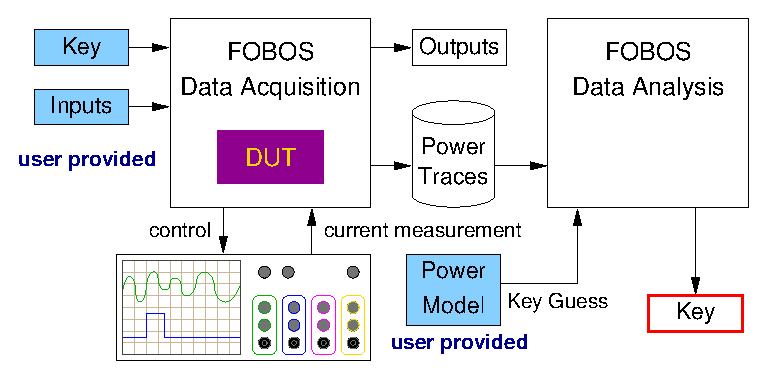
\includegraphics[scale=0.8]{figures/fobos-top}
\caption{\label{fig:fobos-top}Components of FOBOS}
\end{center} 
\vspace{-3ex}
\end{figure}

Figure~\ref{fig:fobos-top} shows various components of FOBOS. It consists of the 
\emph{FOBOS Hardware} as well as software for \emph{Data Acquisition and Control} 
and \emph{Data Analysis}. The FOBOS Hardware consists of two FPGA boards that 
are connected to each other. It is also possible to use the SASEBO GII board instead.
The user has to provide the hardware description of the
cipher under investigation, the key, a set of inputs and a power model. 
The Data Acquisition and Control module configures and controls the 
FOBOS Hardware and the Oscilloscope.  It takes the user provided key and
inputs and sends them to the FOBOS Hardware which in turn encrypts the inputs 
with the key and returns the outputs (i.e.\ ciphertext). As soon as the FOBOS 
Hardware starts with the encryption, it sends a trigger signal to start data
acquisition of the oscilloscope.  The Data Analysis module uses the user 
supplied power model, which can be based on inputs and/or outputs, and the 
power traces collected by the oscilloscope to recover the key. 


%FOBOS uses a set of scripts written in perl, to automate the process of data transmission 
%and collection between the PC and the control board. The scripts are controlled by
%two files, \emph{config.txt} \& \emph{osc\_config.txt}. The \emph{config.txt} file
%contains the option values to control the operation of FOBOS, while the \emph{osc\_config.txt}
%contains the settings for the oscilloscope. The \emph{Inputs} or plaintext, \emph{Key}
%and the \emph{Outputs} obtained from the crypto computations are in the hex format.




%%%%%%%%%%%%%%%%%%%%%%%%%%%%%%%%%%%%%%%%%%%%%
\section{Architecture of FOBOS}
FOBOS has two parts, the \emph{FOBOS Hardware} and the \emph{FOBOS Software}. 
The following sections describe the functionality of various components of FOBOS.

\subsection{FOBOS Hardware}
A schematic diagram of the FOBOS 
hardware is shown in Fig.~\ref{fig:fobos-block}. It consists of
two boards~\textit{Victim Board} \& \textit{Control Board} connected together by 
the so called bridge connector.
The cryptographic algorithms whose security needs to be evaluated are to be implemented on 
the FPGA of the Victim board. Data i.e.\ plaintext and/or key is sent from the PC 
via USB to the control FPGA, which then forwards the data to the Victim FPGA. After 
processing, the Victim FPGA sends the results back to the Control FPGA which in turn 
forwards the results to the PC for verification. The control board also sends a 
trigger signal to the oscilloscope to capture power measurement data. 
%
\begin{figure}[t]
\begin{center}
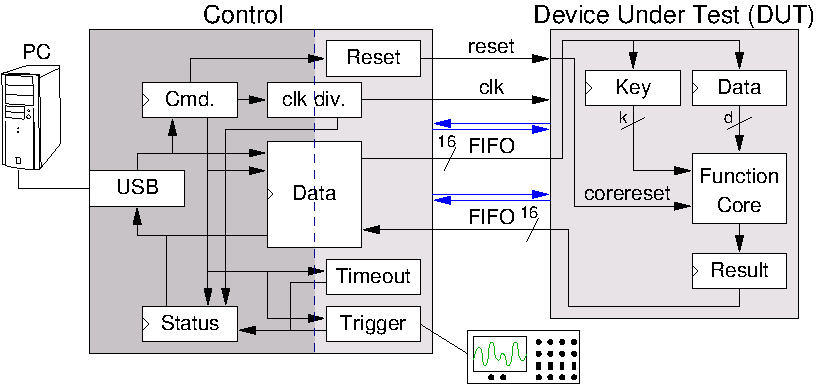
\includegraphics[scale=0.8]{figures/fobos-block}
\caption{Schematic Diagram of FOBOS Hardware}\label{fig:fobos-block}
\end{center} 
%\vspace{-3ex}
\end{figure}
%


\textbf{Control Board:}
The control board used by FOBOS is either a Nexys2 or a Nexys3 board.  
Table~\ref{tab:fobos-cntrlbd} shows details of the both boards. 
%Currently our FOBOS prototype only supports the Nexys2. 
The control board contains
several modules (see Fig.~\ref{fig:fobos-block}) and two clock domains.
It uses the on-board 50\,MHz oscillator as base clock for the USB communication.
The second clock is generated through a clock divider circuit which uses
the Digital Clock Managers (DCMs) to generate a clock in the range of 
350\,KHz $\sim$ 50\,MHz from the 50\,MHz oscillator on board depending upon the user's choice and the 
oscilloscope specification.  This clock is used for communication with the victim FPGA 
and also provided to the victim FPGA board.

\begin{table}[ht]%
%  \vspace{-2ex}%
  \centering%
  \caption{FOBOS FPGA Control Boards}%
  \label{tab:fobos-cntrlbd}%
%  \small%
  \begin{tabular}{|l|l|r|l|l|r|}\hline
  {Board}      & {FPGA}       & {Technology}  & {Connector} & {PC-Control} & {Cost}\\ \hline
  Nexys 2    & Spartan-3E & 90 nm       & Hirose FX2 (43) & USB2       &\$149\\ 
  Nexys 3    & Spartan 6  & 45 nm       & VHDC (40)       & USB2       &\$199\\ \hline
  \end{tabular}%
  \vspace{-2ex}%
\end{table}

The control board receives commands from the PC and returns a status. This is facilitated
through the 8-bit Command and Status registers. We use them to implement a simple 
protocol between PC and Control FPGA which is explained in Section \,~\ref{pcccp}. 

The Trigger module generates a reference point from which the oscilloscope should 
start measuring the power consumption of the victim FPGA. Depending upon the
user's requirement, this reference point can be set through a command to the 
beginning of the cryptographic operation or to specific clock cycle during the computation. 
This reference point is later used to perform signal alignment of several power traces.

A Timeout module makes sure that PC receives a status (of TIMEOUT) if an exception occurs 
during the communication with the victim or if the victim does not respond within a given 
time. This timeout value can be specified through a command. The timeout counter is
automatically reset each time the victim returns data.

The Reset module is used to send a reset signal to the crypto core implemented on the victim FPGA
depending upon the value specified by the user. This is useful if for example a cryptographic
operation takes 1,000 clock cycles to complete, however, the interesting event happens in the
30th clock cycle. The user can then reset the victim automatically every 35 clock cycles
and start a new encryption without having to wait for the encryption to complete.

\textbf{Victim Board:} We are investigating several FPGA boards available 
in the market, which can be used as Victim boards for FOBOS. Table~\ref{tab:fobosvictim} 
shows some potential Victim boards. The column ``$\mathrm{V_{Core}}$ Jumper''  
indicates whether the board contains a jumper on the core power line which allows for
by-passing the on board core power supply and inserting a current sensor (resistor or 
current probe) to measure the power consumption of the victim FPGA. 
So far, we have successfully used the Spartan 3E Starter Kit, Spartan 3E-1600 Developer 
Board, and the Altera DE1 board as FOBOS Victim boards. As the Altera DE1 does not have
$\mathrm{V_{Core}}$ Jumper, we had to de-solder the voltage regulator for core voltage.
On all boards we also removed several capacitors.
Our preliminary investigation (shown in Table~\ref{tab:fobosvictim}) into the 
other boards have shown that it is possible to modify them
in order to measure the current of the core supply.

\begin{table}[ht]%
 \vspace{-2ex}%
  \centering%
  \caption{FOBOS FPGA victims}%
  \label{tab:fobosvictim}%
%  \small%
  \begin{tabular}{|l|l|r|c|l|r|}\hline
                        &               &{Techn-}&{$\mathbf{V_{Core}}$}        &   \\
  {{Board}}       & {{FPGA}}&{ology} &{Jumper}    & {{Cost}}\\ \hline
  Spartan 3E Starter    & Spartan-3E    & 90\,nm & yes        & \$159\\
  Spartan 3E-1600 Dvlp. & Spartan-3E    & 90\,nm & yes        & \$225\\
  Altera DE1            & Cyclone-II    & 90\,nm & no         & \$150\\
  Cyclone III Starter   & Cyclone-III   & 65\,nm & yes        & \$199\\ 
  Genesys Board         & Virtex-5      & 65\,nm & no         & \$449\\
  Altera DE2-115        & Cyclone-IV    & 60\,nm & no         & \$299\\
  Altys Board           & Spartan-6     & 45\,nm & no         & \$199\\
  Altera DE4            & Stratix-IV    & 40\,nm & no         & \$2,995\\
  Xilinx ML605          & Virtex-6      & 40\,nm & no         & \$1,795\\
  Xilinx KC705          & Virtex-7      & 28\,nm & no         & \$1,695\\
%  Xilinx Zynq-7000      & Zynq          & 28\,nm & no         & \$895\\
  %Altera DE3            & Stratix-3     & 65\,nm &            & \$2695\\
\hline
  \end{tabular}%
  \vspace{-3ex}%
\end{table}

For each victim board we plan on publishing instructions on how to modify it for DPA
and the printed circuit board (PCB) layout of the bridge connector which connects
the victim board securely to the control board.

% \subsubsection{Bridge Connector:}
% The bride connector is a PCB with connectors that securely connect the victim board 
% to the control board. The bridge connector also has an SMA port which can be used 
% to supply a clock from an external source to both control and victim boards.

\textbf{FOBOS Control-Victim Protocol}
%
The FOBOS Control-Victim Protocol uses a simple FIFO interface to transfer data 
to and from the control and victim FPGAs.  The functionality of the input and output 
ports of the protocol is described in~\cite{1458},~\cite{GHR10}.
%
\begin{figure}[ht]
\begin{center}
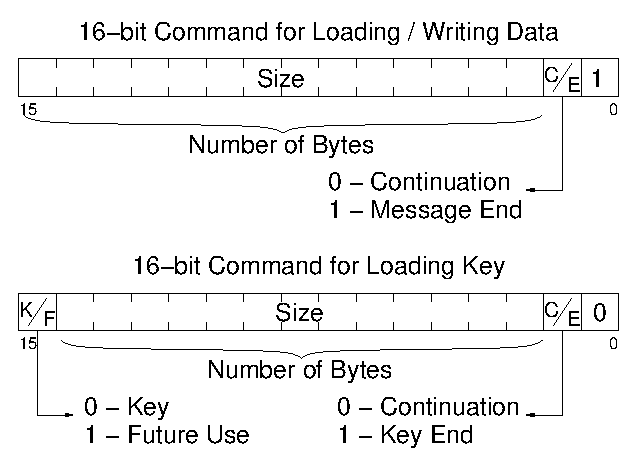
\includegraphics[scale=0.7]{figures/protocol}
\caption{\label{fig:protocol}FOBOS Protocol}
\end{center} 
  \vspace{-3ex}%
\end{figure}
%
All data and key to and from the FPGA is broken into segments.
The first 2 bytes (16-bit) of each segment is a command word, which decides the nature 
of the segment and the number of bytes being sent. The format of the 16-bit command words 
is shown in Fig~\ref{fig:protocol}. A `0' value in the LSB and a `0' value in the MSB 
of the command word indicates that a key is being sent. 
Similarly a `1' value in the LSB indicates that data is send. The bit in position `1' 
indicates with a `0' that more segments are following the current one, a `1' indicates
that the current segment is the last.
The MSB bit value `1' for a 16-bit command for loading the key is left explicitly 
for future use.
This protocol does not require the control board to know what the block size of the
cryptographic function is.
The widths of the buses for `k' and data `d' indicated in Fig~\ref{fig:fobos-block} can be 
defined by the user according to the requirement of the cryptographic implementation. 

\subsection{FOBOS Software}
%
\textbf{FOBOS Software Control Flow:}
The FOBOS control flow is shown in Fig.~\ref{fig:fobos-ctrlflow}. The control script
parses the configuration files and initializes the FOBOS
environment. It performs a simple tool check to verify whether the necessary
library files essential for data transfer and oscilloscope control are 
installed and only continues when the check passes successfully. The control script 
then assigns the hardware and oscilloscope attribute values as specified by the user 
in the configuration files. The FOBOS hardware then performs a built-in self test to
check whether all the attributes are set accordingly and issues an appropriate 
status message to the control script. The status message can be a success or an error 
code. If the control receives an error code it exits the program displaying proper error message.
On receiving a success code, the control script instructs the oscilloscope to digitize
its analog inputs which then in turn waits for the trigger 
signal from the control board to start capturing data.
The plaintext and the key are then transferred to the FOBOS hardware and the control
script waits until it receives data from the oscilloscope. Once the oscilloscope data 
is captured, the control script writes the outputs from the FOBOS hardware to a file.
\begin{figure}[ht]
\begin{center}
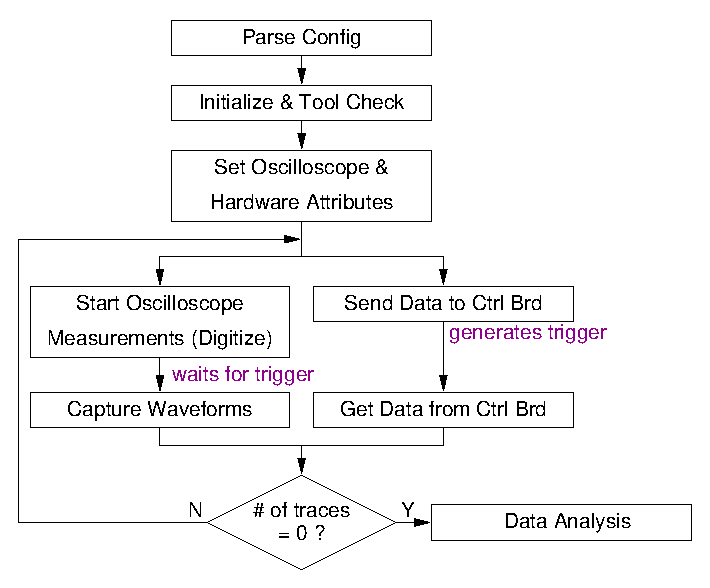
\includegraphics[scale=0.8]{figures/data_acq}
\caption{\label{fig:fobos-ctrlflow}FOBOS Control Flow}
\end{center} 
\vspace{-3ex}
\end{figure}

FOBOS has support for two data capturing modes, called \emph{Single Capture} and \emph{Multi Capture}
to capture the power traces. Single Capture mode, as shown in Fig.~\ref{fig:fobos-captmet}a), assumes that
a power trace contains a single encryption whereas Multi Capture mode, as shown in 
Fig.~\ref{fig:fobos-captmet}b), contains multiple encryptions per power trace. 
Once all data has been captured the control is transferred to data analysis module.  

\textbf{FOBOS PC- Control Communication Protocol:}~\label{pcccp}
%User also has the option of using a configuration file to specify the parameters.
FOBOS uses the command \& status registers to control the PC- Control communication.
The command register is used (shown in Fig.~\ref{fig:fobos-block}) to pass the 
option values to the modules inside the control FPGA and 
to signal the control board that PC is ready to transmit the data.
The status register (shown in Fig.~\ref{fig:fobos-block}) on the other hand, is used for
signaling the PC that the control FPGA is ready to transmit the data obtained from 
victim FPGA or to report errors. 
\begin{figure}[ht]
\begin{center}
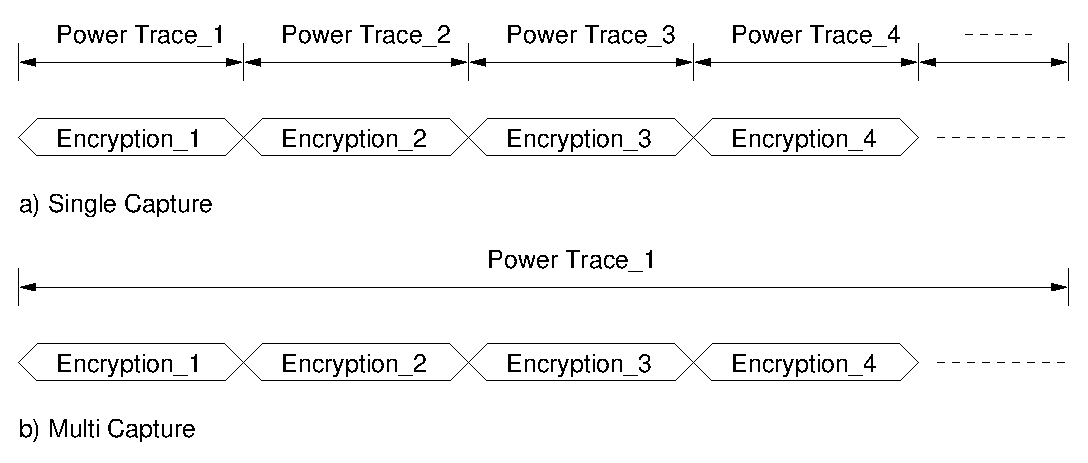
\includegraphics[scale=0.6]{figures/capture_methods}
\caption{\label{fig:fobos-captmet}Capture Modes}
\end{center} 
\vspace{-3ex}
\end{figure}

\textbf{FOBOS Data Acquisition Module:}
The data acquisition module configures the oscilloscope and retrieves its data.
Its behaviour is determined by a configuration file which uses a generic,
oscilloscope brand independent description. A special, oscilloscope dependent
sub-module translates the configuration file to commands which are oscilloscope specific. 
The sub-module of our prototype uses the Virtual Instrument Software Architecture (VISA) 
library which is a standard for configuring and programming instruments using a
variety of interfaces.
Presently, the FOBOS prototype supports communication for oscilloscopes from Agilent 
Technologies. In future we plan to provide support for oscilloscopes from other
manufacturers.

\section{FOBOS Data Analysis Module:}
The Data Analysis module consists of 3 sub-modules as shown below:
\begin{itemize}
\item Signal Alignment Module
\item Post processing Module
\item SCA Module
\item Statistics Module
\end{itemize}

\subsection{Signal Alignment Module}
As the name indicates, the main function of this module is to align all the measured power traces
with respect to time using a reference signal called the "Trigger" signal. Depending upon the type
of capture mode used i.e. Single capture or Multi capture its functionality varies. In Single capture
mode as each measurement trace contains only one encryption, the power traces are aligned when the 
"Trigger" signal becomes logic high. In the Multi capture mode, as each measurement trace contains 
multiple encryptions, the start of each encryption is indicates by the Trigger signal.
To be exact, the measurement point from one trigger high to the subsequent trigger high is equivalent
to one encryption. The measurement module chops up the trace accordingly and aligns them.

\subsection{Post processing Module}
Currently FOBOS supports three Post processing sub modules. They are:
\begin{enumerate}
\item Sample Space Disposition
\item Compression
\item Trace Expunge
\end{enumerate}

\textbf{Space Disposition} allows user to select a part of the trace to perform further post processing
or to perform statistical testing. This also reduces computation time during statistical testing.

\begin{figure}[ht]
\begin{center}
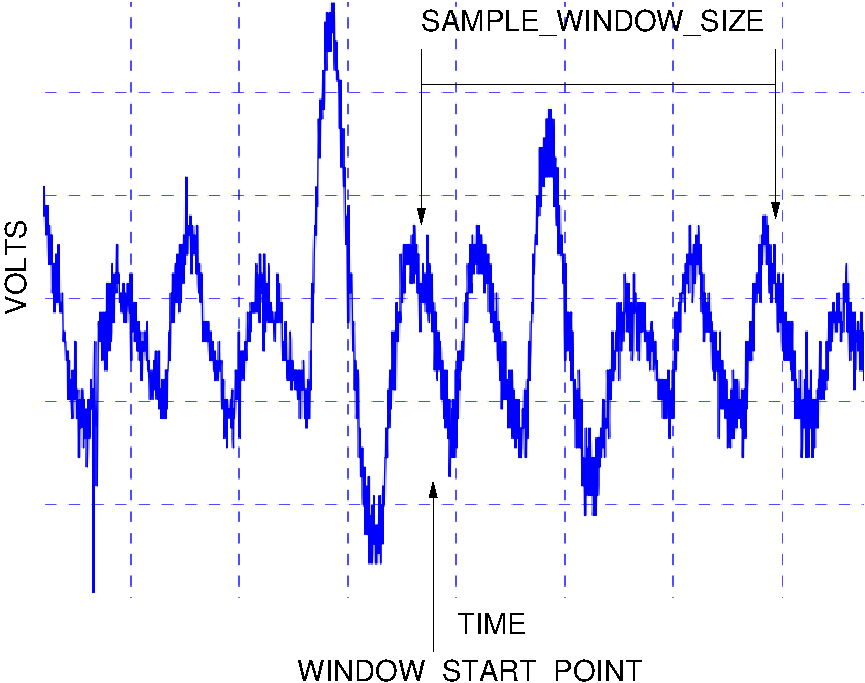
\includegraphics[scale=0.6]{figures/sampleSpaceDisp}
\caption{\label{fig:ssd}Sample Space Disposition}
\end{center} 
\vspace{-3ex}
\end{figure}

The parameters which facilitate this selection are "WINDOW START POINT" and "SAMPLE WINDOW SIZE". As shown in
Fig~\ref{fig:ssd} "WINDOW START POINT" parameter indicate which point in time to further sample the trace and the
"SAMPLE WINDOW SIZE" parameter indicates the number of points to be sampled and stored to a new trace.

\textbf{Compression} allows user compress the power trace in chunks or as a whole
depending upon the user requirement by using the "COMPRESSION LENGTH" parameter as shown in Fig~\ref{fig:cmp}
The user can also the type of compression to be used. They are:
\begin{itemize}
\item Max: Can compress the user specified sample size to the maximum of the given sample set.
\item Min: Can compress the user specified sample size to the minimum of the given sample set.
\item Mean: Can compress the user specified sample size to the average of the given sample set.
\end{itemize}

This also reduces computation time during statistical testing.

\begin{figure}[ht]
\begin{center}
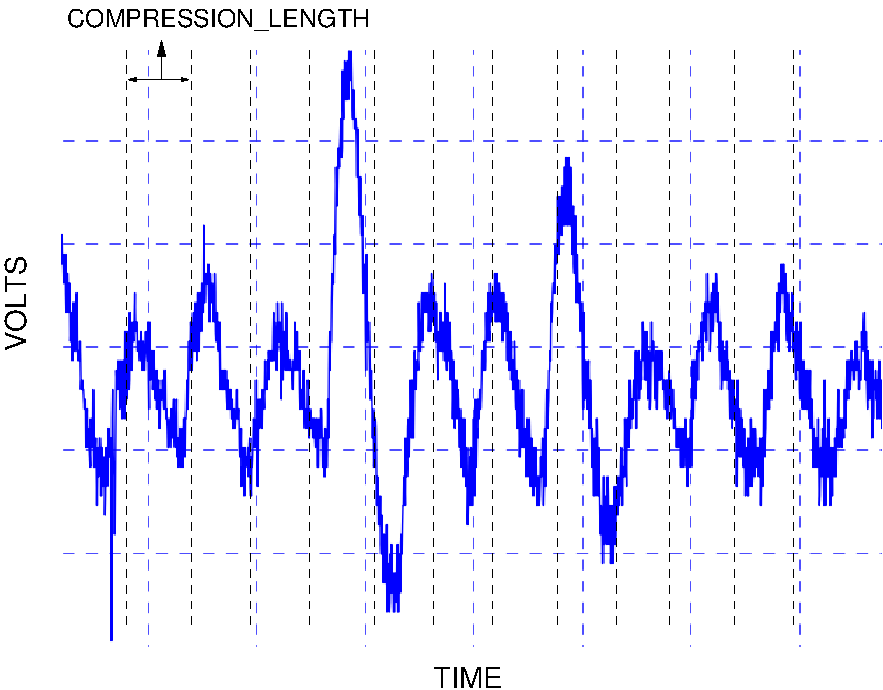
\includegraphics[scale=0.6]{figures/compression}
\caption{\label{fig:cmp}Compression}
\end{center} 
\vspace{-3ex}
\end{figure}

\textbf{Trace Expunge} allows user to selectively "expunge" or discard one or more traces 
depending upon two different selection criteria:

\begin{itemize}
\item Variance: User specifies Upper and Lower bound values. A given trace is removed if its variance (of the entire trace)
is above upper limit or below lower limit.
\item Standard Deviation: User specifies Upper and Lower bound values. A given trace is removed if its standard 
deviation (of the entire trace) is above upper limit or below lower limit.
\end{itemize}

\begin{figure}[ht]
\begin{center}
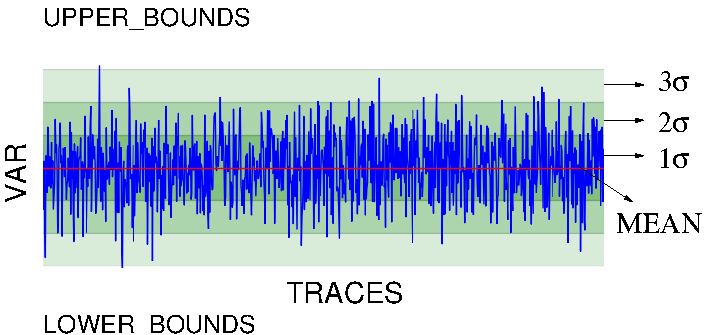
\includegraphics[scale=0.6]{figures/traceExpungMod}
\caption{\label{fig:tex}Trace Expunge}
\end{center} 
\vspace{-3ex}
\end{figure}

This will help in removing traces which are heavily influenced by factors like measurement artefacts etc,.

\subsection{SCA Module}
Currently FOBOS supports following Side-channel distinguishers:
\begin{itemize}
\item Pearson's r
\item Spearman's RHO
\end{itemize}
\textbf{Pearson's r}
We assume a linear relationship between the power consumption of the device
and the data being processed. Hence we use Pearson product-moment correlation
coefficient (r), commonly known as Pearson's correlation to correlate instantaneous power
consumption with hamming distance model~\cite{1203}.

The Pearson's correlation (r) between the the power consumption of the device P and the
hypothetical power model H is given by the Eq.~\ref{eq:pearsons-r}

\begin{equation}\label{eq:pearsons-r}
r(P,H) =\frac{n \sum_{i}^{n}{P_iH_i}-\sum_{i}^{n} P_i\sum_{i}^{n}H_i}{\sqrt{n\sum_{i}^{n} 
	      P_i^2-(\sum_{i}^{n} P_i)^2}\sqrt {n\sum_{i}^{n} H_i^2-(\sum_{i}^{n} H_i)^2}}
\end{equation}   

Correlation Power Analysis (CPA) is a form of DPA where we use a different statistical test to obtain the secret key. Henceforth, we use
the term DPA and CPA alternatively throughout this document.

\textbf{Spearman Rank coefficient}, on the other hand, is a measure of monotonic relationship 
between two variables, in this case between power consumption and power model.
The Rank correlation between power consumption samples P and power consumption hypothesis samples G is given by
\begin{equation}
\label{pceqn}
RHO(P,G)=1-\frac{6\sum_{i}^{n}d_i^2}{n(n^2-1)}
\end{equation} 
where $d_i$ =$P_i$ - $G_i$, and $P_i$, $G_i$ are ranks of the variables P and G 

\subsection{Statistics Module}
FOBOS currently supports following statistic functions.
\begin{itemize}
\item Mean : Calculates mean of the trace, both trace and sample wise, as shown in Fig~\ref{fig:tvs}.
\item Standard Deviation : Calculates Standard Deviation of the trace, both trace and sample wise, as shown in Fig~\ref{fig:tvs}.
\item Variance : Calculates Variance of the trace, both trace and sample wise, as shown in Fig~\ref{fig:tvs}.
\end{itemize}

\begin{figure}[ht]
\begin{center}
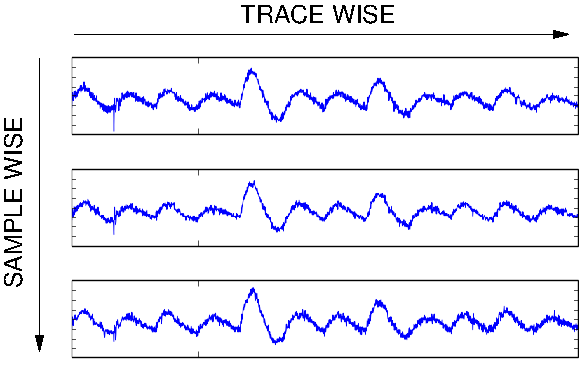
\includegraphics[scale=0.6]{figures/sampleVstrace}
\caption{\label{fig:tvs}Trace wise vs Sample wise}
\end{center} 
\vspace{-3ex}
\end{figure}


\section{CPA Attack on AES using FOBOS}

This section describes a Correlation Power Analysis (CPA) attack of an implementation of the
Advanced Encryption Standard (AES)~\cite{146} using FOBOS. 
AES is an symmetric-key cipher used extensively
in security sensitive applications world wide. AES applies four different transformations,
SubBytes, ShiftRows, MixColumns, and AddRoundKey, per round and iterates through several 
such rounds depending upon the key size. An intermediate key called 
"round key" is generated and used per round which is derived from the original key through 
a reversible key scheduling function. We have implemented a basic iterative architecture i
of AES with 128-bit 
key length and 128-bit wide datapath requiring 11 clock cycles for one encryption.
Key scheduling is done on-the-fly and the SubBytes function is realized through look-up-tables.
The block diagram for this design is shown in Fig.~\ref{fig:fobos-aes128}.

\begin{figure}[ht]
\begin{center}
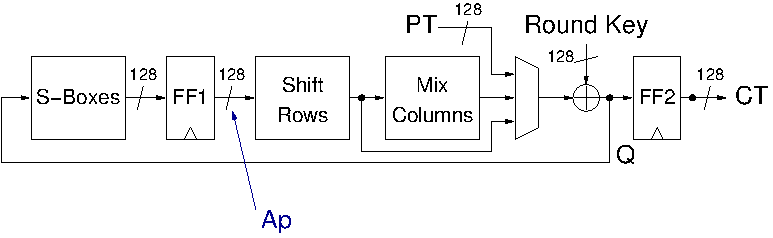
\includegraphics[scale=0.8]{figures/aes128}
\caption{Block Diagram of the AES Core}\label{fig:fobos-aes128}
\end{center} 
\vspace{-3ex}
\end{figure}

We attack our AES design during the first round at the output of the register \textsf{FF1} 
indicated by \textsf{Ap} in Fig.~\ref{fig:fobos-aes128}.
%In order to decrease the loading time of the new plaintext (PT), we reuse the ciphertext (CT)
%as the PT for the next encryption. 
The equation for calculating the Hamming Distance (HD) is shown 
in~\ref{eq:hamm-aes}. We use Pearson's Correlation to correlate the instantaneous
power consumption with the HD model. 

\begin{equation}\label{eq:hamm-aes}%
P_{est.} = \mathrm{HD}(\mathrm{SBOX}(CT_{i}), \mathrm{SBOX}(k_{guess} \oplus PT_{i+1}))
\end{equation}


\begin{figure}[ht]
\begin{center}
\includegraphics[scale=0.8]{figures/victimwrapper}
\caption{\label{fig:fobos-vicaes128}AES Core with Wrapper on Victim FPGA}
\end{center} 
\vspace{-3ex}
\end{figure}

Figure~\ref{fig:fobos-hardattb} shows a snippet of hardware attributes
specified in the FOBOS configuration file. FOBOS Control sends data from datain.txt 
and a key from keyin.txt, which are both in
the format of ASCII coded Hexadecimal values, to the victim. A snapshot of these files
is shown in Fig.~\ref{fig:fobos-iof}. FOBOS Control sets the timeout
to 30,000 clock cycles and the trigger to 4 clock cycles after processing starts.
The victim clock is set to run at 500\,KHz and the result will be 
stored in hexadecimal values in the file outputs.txt
% which is located in the corresponding project folder.

\begin{figure}[ht]
\begin{Verbatim}[frame=single]
DATA_FILE = datain.txt
KEY_FILE  = keyin.txt
CLK_FREQ = 500 KHz 
TIME_OUT = 30000
TRIGGER = 4
CAPTURE_MODE = multi
\end{Verbatim}
\caption{\label{fig:fobos-hardattb}Snippet of config.txt}
\end{figure}


\begin{figure}[H]
\begin{Verbatim}[frame=single]
. . . .
40 F6 BB C7 94 78 0B D7 99 C3 5F 6A 77 8F 05 D8 
A5 34 8B CC 02 EE C0 68 B4 9E 29 A5 22 B8 EF 54 
CB 00 B7 22 F8 36 F9 E4 40 E2 EE BD 1B 13 BA A3
. . . .
\end{Verbatim}
\begin{Verbatim}[frame=single]
2B 7E 15 16 28 AE D2 A6 AB F7 15 88 09 CF 4F 3C
\end{Verbatim}
\begin{Verbatim}[frame=single]
. . . .
0A 59 8B A5 3D B3 0D B6 34 B2 C2 7E 98 A8 DB 71 
2E 13 7A 5F E2 F9 86 C0 15 9A 69 AB 6E 3F 04 01 
FB D0 09 43 E7 71 59 4A 15 37 53 33 A3 EF 74 1B 
. . . .
\end{Verbatim}
\caption{\label{fig:fobos-iof}Plaintext, Key \& Ciphertext sent to FOBOS in hex format}
\end{figure}

A snippet of oscilloscope attributes from osc\_config.txt file is shown in Fig.~\ref{fig:fobos:osccon}.
The FOBOS control connects to the instrument specified by the VISA address from the RESOURCE attribute.
The voltage ranges of the channels of the oscilloscope are specified in terms of vertical full-scale 
value in volts. The time range of the channels are specified in terms of horizontal full-scale
value in seconds. In general oscilloscopes are configured in 8x10 graticule, therefore channel-1 range 
is 0.0125 Volts/div, channel-2 range is set to 2 Volts/div. The time range is set to 0.01 Sec/div. We also set
the trigger source to be channel-2 and the condition on trigger to be positive edge.

\begin{figure}[H]
\begin{Verbatim}[frame=single]
RESOURCE  = GPIB0::7::INSTR    #Instrument Resource
CHANNEL_RANGE1 = 0.1V          #Specified in Volts per screen
CHANNEL_RANGE2 = 16V           #Specified in Volts per screen
TIME_RANGE = 0.001             #Specified in seconds per screen
TRIGGER_SOURCE =  CHANNEL2
TRIGGER_MODE =  EDGE  
TRIGGER_SLOPE = POSITIVE
\end{Verbatim}
\caption{\label{fig:fobos:osccon}Snippet of osc\_config.txt}
\end{figure}

The FOBOS control sends the data from the oscilloscope i.e.\ the power traces, inputs, and outputs to
the data analysis module. The first step involves processing the raw 
power trace using the preamble information to obtain the \emph{measured\_power\_trace}.
We use Multi Capture mode to obtain the Raw power trace. We use the Signal alignment 
module to process and align the traces as shown in Fig.~\ref{fig:alpt}


\begin{figure}[H]
\begin{center}
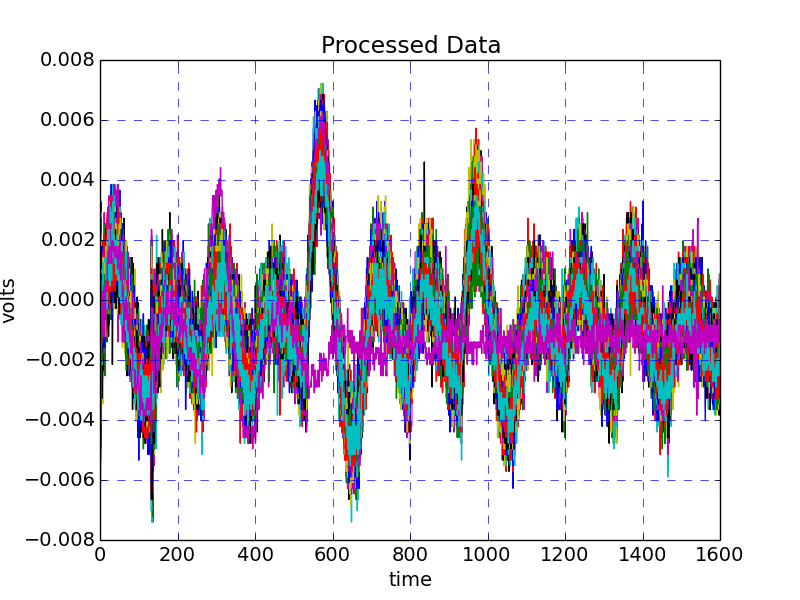
\includegraphics[scale=0.8]{figures/scaTrace1}
\caption{\label{fig:alpt}Aligned Power Trace}
\end{center} 
\vspace{-3ex}
\end{figure}

The parameters used for the signal processing module is shown in Fig.~\ref{fig:fobos:paramsa}.

\begin{figure}[H]
\begin{Verbatim}[frame=single]
CAPTURE_MODE = MULTI # MULTI|SINGLE
TRIGGER_THRESHOLD = 1.8
TRACE_EXPUNGE_PARAMS = VAR:0.0000025:0.0000035
SAMPLE_WINDOW = 1000
WINDOW_START_POINT = 100
COMPRESSION_LENGTH = 40
COMPRESSION_TYPE = MAX
\end{Verbatim}
\caption{\label{fig:fobos:paramsa}Snippet of Signal Processing module Parameters}
\end{figure}


We perform Trace Expunge sub routine on the processed power traces
using the parameters shown in Fig.~\ref{fig:fobos:paramsa}. The resultant power trace is
shown in Fig.~\ref{fig:pttx}

\begin{figure}[H]
\begin{center}
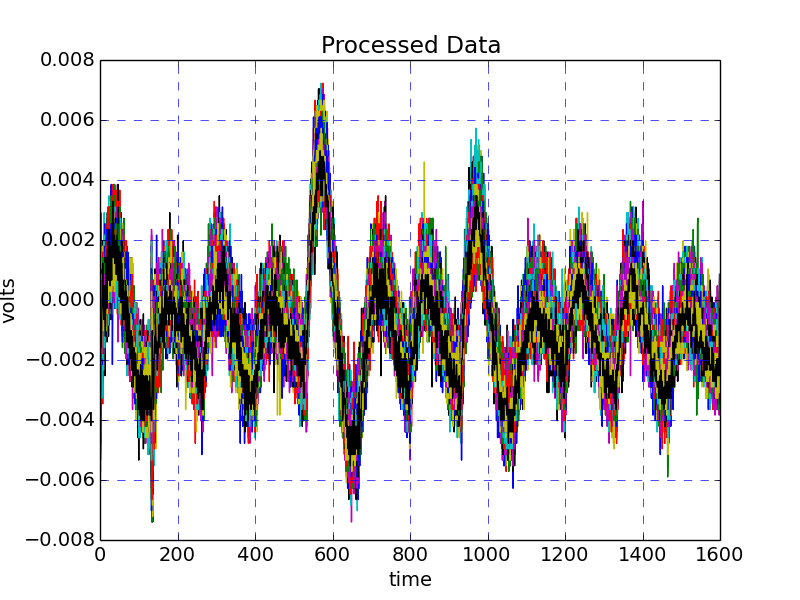
\includegraphics[scale=0.8]{figures/scaTrace2}
\caption{\label{fig:pttx}Power Trace after Trace Expunge}
\end{center} 
\vspace{-3ex}
\end{figure}

We further process the resultant power trace using sample space disposition and compression
using the parameters shown in Fig.~\ref{fig:fobos:paramsa}.
 The resultant
power traces are shown in Fig.~\ref{fig:ptsp} and Fig.~\ref{fig:ptcp}

\begin{figure}[H]
\begin{center}
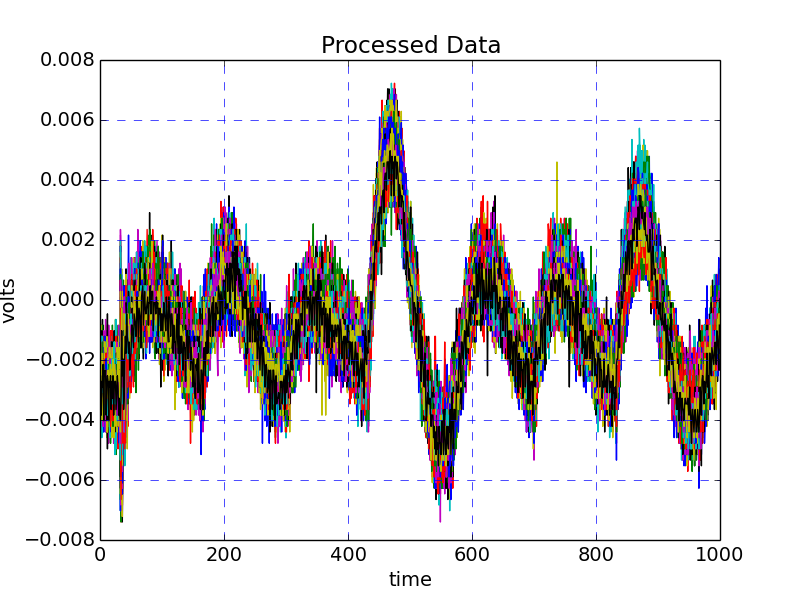
\includegraphics[scale=0.8]{figures/scaTrace3}
\caption{\label{fig:ptsp}Power Trace after Sample Space Disposition}
\end{center} 
\vspace{-3ex}
\end{figure}

\begin{figure}[H]
\begin{center}
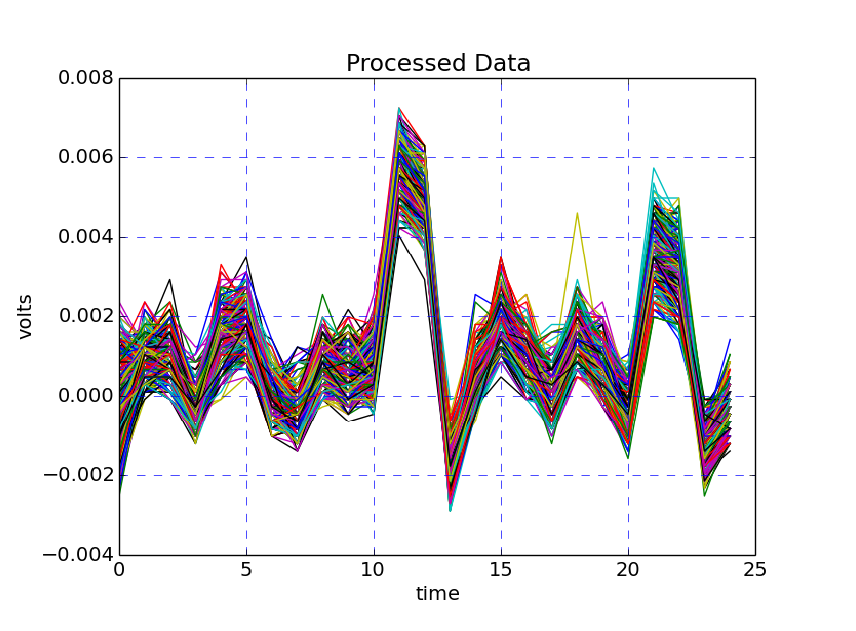
\includegraphics[scale=0.8]{figures/scaTrace4}
\caption{\label{fig:ptcp}Power Trace after Compression}
\end{center} 
\vspace{-3ex}
\end{figure}

The CPA attack is conducted on a sub-byte of the key depending upon the user choice. Hence 
there are 256 different key guess values and correspondingly 9 different HD values i.e.\ 0 $\rightarrow$ 8.
A snippet of the \emph{est\_power\_traces} per key guess value is shown in Fig~\ref{fig:fobos-estpower}. 
\begin{figure}[ht]
\begin{Verbatim}[frame=single]
4 6 3 4 5 1 5 4 4 2 4 3 5 6 3 4 4 3 4 2 . . . .
3 2 7 6 5 6 5 5 7 3 5 4 4 2 6 5 2 3 2 5 . . . .
5 4 3 6 4 5 3 4 3 3 6 5 3 0 2 5 6 5 6 5 . . . .
. . . .
\end{Verbatim}
\caption{\label{fig:fobos-estpower}Hypothetical Power Model}
\end{figure}

The sca module than calculates the Pearson's Correlation and Spearman's Rank correlation
for all the key guesses by correlating 
the \emph{est\_power\_traces} and \emph{processed\_power\_trace}. 
Snippets of the output logs of the Pearson's and Spearman's Correlation are shown
in Fig.~\ref{fig:pearson} and Fig.~\ref{fig:spearman} respectively.

\begin{figure}[H]
\begin{Verbatim}[frame=single]
Window[0] Key Byte- 0x5d [93] Correlation- 0.080
Window[1] Key Byte- 0x9c [156] Correlation- 0.078
Window[2] Key Byte- 0x9c [156] Correlation- 0.086
Window[3] Key Byte- 0x6 [6] Correlation- 0.086
Window[4] Key Byte- 0x16 [22] Correlation- 0.109
Window[5] Key Byte- 0x16 [22] Correlation- 0.175
Window[6] Key Byte- 0xa3 [163] Correlation- 0.087
Window[7] Key Byte- 0xd7 [215] Correlation- 0.082
\end{Verbatim}
\caption{\label{fig:pearson}CPA using Pearson's r Log file}
\end{figure}

\begin{figure}[h]
\begin{Verbatim}[frame=single]
Window[0] Key Byte- 0x5d [93] Correlation- 0.082
Window[1] Key Byte- 0x9c [156] Correlation- 0.083
Window[2] Key Byte- 0x78 [120] Correlation- 0.109
Window[3] Key Byte- 0x6 [6] Correlation- 0.083
Window[4] Key Byte- 0x16 [22] Correlation- 0.105
Window[5] Key Byte- 0x16 [22] Correlation- 0.176
Window[6] Key Byte- 0xa3 [163] Correlation- 0.086
Window[7] Key Byte- 0xd7 [215] Correlation- 0.091
\end{Verbatim}
\caption{\label{fig:spearman}CPA using Spearman's RHO Log file }
\end{figure}

The sca module also plots two graphs, called the Correlation Plot 
shown in Fig.~\ref{fig:prcorrplt} for Pearson's r and Fig.~\ref{fig:spcorrplt} for 
Spearman's RHO respectively.  
The correlation plot shows how well each individual key guess correlates with the power trace.
The peak value of this plot indicates the correct sub-key byte. 

\begin{figure}[H]
\begin{center}
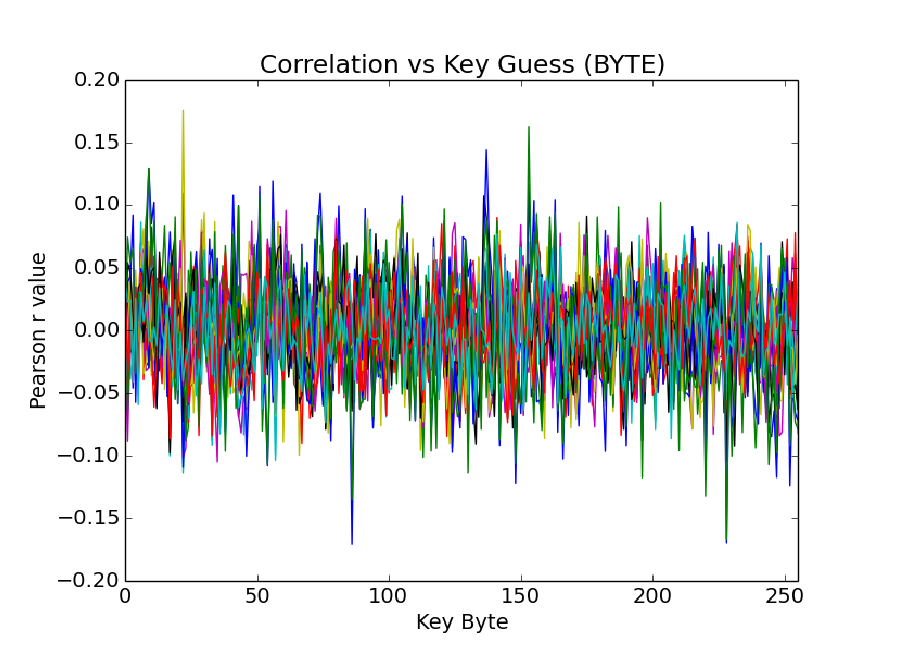
\includegraphics[scale=0.8]{figures/pearson-r}
\caption{\label{fig:prcorrplt}Results of Pearson's r}
\end{center} 
\vspace{-3ex}
\end{figure}

\begin{figure}[H]
\begin{center}
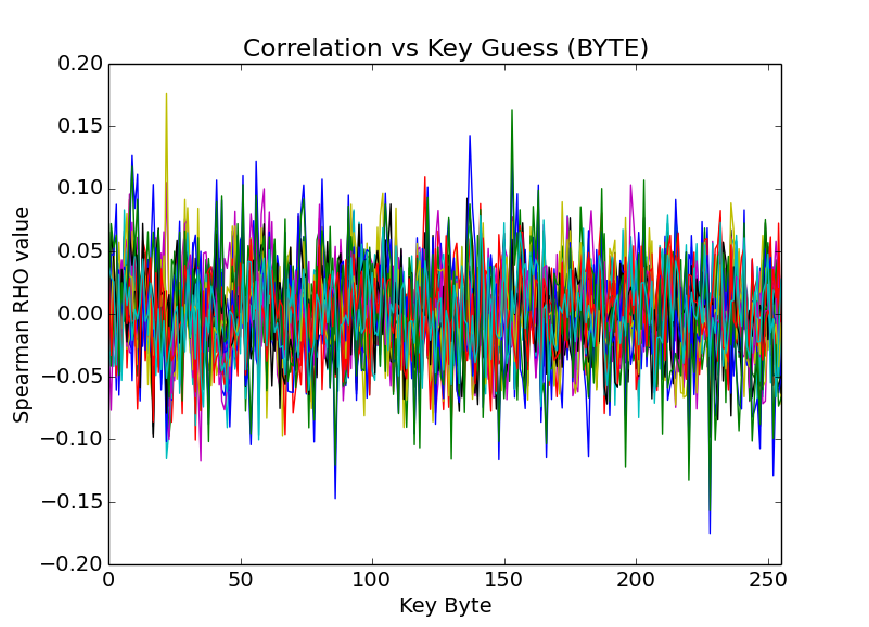
\includegraphics[scale=0.8]{figures/spearman-rho}
\caption{\label{fig:spcorrplt}{Results of Spearman's RHO}}
\end{center} 
\vspace{-3ex}
\end{figure}

\section{A Step-by-step Guide to Running DPA on the example AES Implementation}

In this section we provide a step-by-step guide to attack the example AES included with FOBOS. We assume that the FOBOS software is installed in the \$fobos directory.
We also assume that Python is installed.

To run DPA attack on the AES implementation provided, follow these steps:
\begin{enumerate}
\item \textbf{Program the control board}
  \begin{enumerate}
  \item Create a new project using Xilinx ISE. In the New Project wizard set the Project Settings as in Fig~\ref{fig:ctrl-design-properties}.
  		\begin{figure}[H]
		\begin{center}
		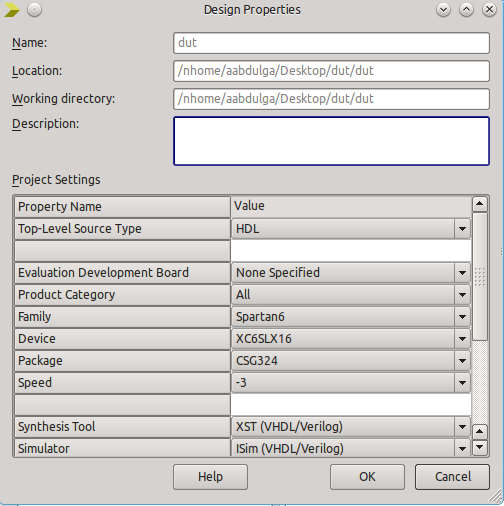
\includegraphics[scale=0.6]{figures/ctrl-design-properties}
		\caption{\label{fig:ctrl-design-properties}FOBOS Controller Desgin Properties}
		\end{center}
		\vspace{-1ex}
		\end{figure}
  \item From the Project menu select Add Source... and add all files from \texttt{\$fobos/sources/common}.
  \item Repeat the previous process to add all files from \texttt{\$fobos/sources/vhdl/control} (add all files except \texttt{Nexys3.ucf}) (See Fig~\ref{fig:ctrl-add-sources}).
		\begin{figure}[H]
		\begin{center}
		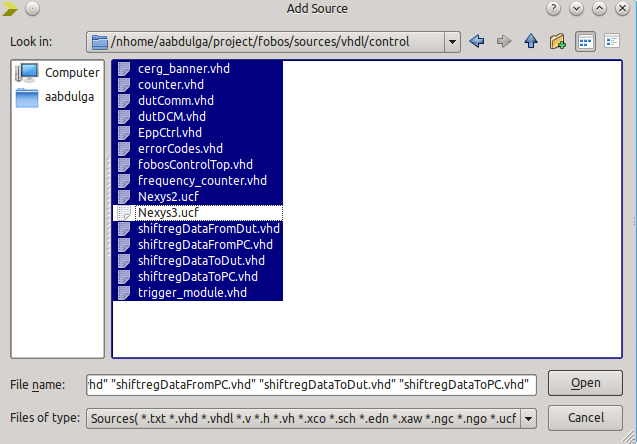
\includegraphics[scale=0.6]{figures/ctrl-add-sources}
		\caption{\label{fig:ctrl-add-sources}Adding Source Files to FOBOS Controller}
		\end{center} 
		\vspace{-1ex}
		\end{figure}
  \item Set the \texttt{fobosControlTopLevel} module as the top-level module for this project (See Fig~\ref{fig:ctrl-set-top-level}).
		\begin{figure}[H]
		\begin{center}
		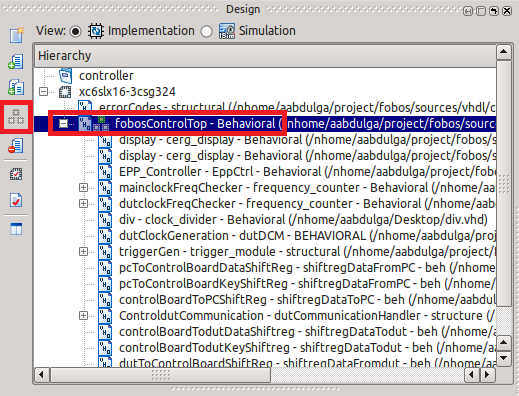
\includegraphics[scale=0.6]{figures/ctrl-set-top-level}
		\caption{\label{fig:ctrl-set-top-level}Setting Top-level Module}
		\end{center} 
		\vspace{-1ex}
		\end{figure}
  \item Generate the programming bit file for the control board by clicking "Generate Programming File" in the Processes window.
  \item Program the control board using Xilinx Impact. In the Processes window, click Configure Target Device (See Fig~\ref{fig:ctrl-run-impact}).
		\begin{figure}[H]
		\begin{center}
		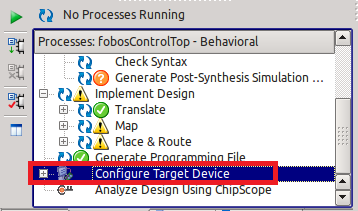
\includegraphics[scale=0.6]{figures/ctrl-run-impact}
		\caption{\label{fig:ctrl-run-impact}}
		\end{center}
		\vspace{-1ex}
		\end{figure}
  \item In the Impact window, click "Boundary Scan" then form the File menu, click "Initialize Chain" and assign the bit file to the FPGA. Now you may right-click the FPGA and click "Program".
		\begin{figure}[H]
		\begin{center}
		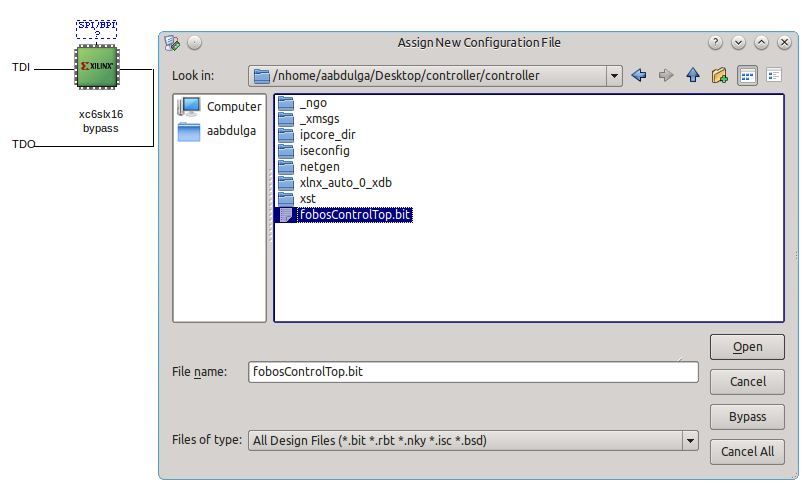
\includegraphics[scale=0.6]{figures/ctrl-program}
		\caption{\label{fig:ctrl-program}Progrmamming Control Board}
		\end{center}
		\vspace{-1ex}
		\end{figure}
  \end{enumerate}
\item \textbf{Program the victim board (DUT)}
  \begin{enumerate}
  \item Create a new project using Xilinx ISE. In the New Project wizard set the Project Settings as in Fig~\ref{fig:dut-design-properties}.
		\begin{figure}[H]
		\begin{center}
		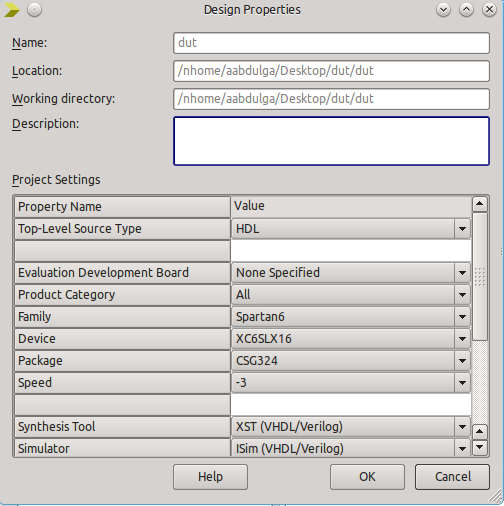
\includegraphics[scale=0.6]{figures/dut-design-properties}
		\caption{\label{fig:dut-design-properties}DUT Design Properties}
		\end{center}
		\vspace{-1ex}
		\end{figure}
  \item From the Project menu select Add Source... and add all files from \texttt{\$fobos/sources/common}.
  \item Repeat the previous process to add all files from \texttt{\$fobos/sources/vhdl/DUT} (add all files except \texttt{Nexys.*}) and all files from \texttt{\$fobos/examples/AES-128/vhdl}  (See Fig~\ref{fig:dut-add-sources}).
		\begin{figure}[H]
		\begin{center}
		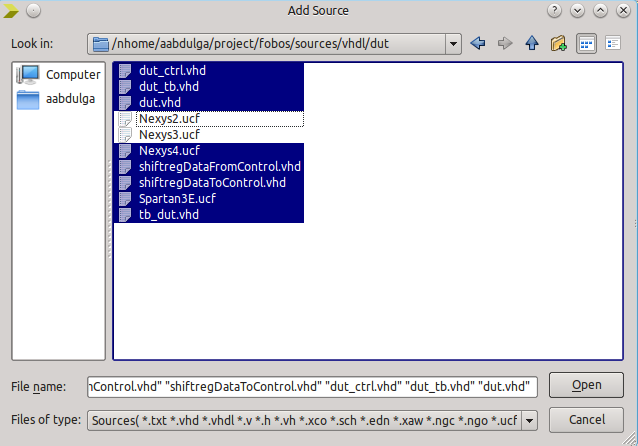
\includegraphics[scale=0.6]{figures/dut-add-sources}
		\caption{\label{fig:dut-add-sources}DUT Add Sources}
		\end{center}
		\vspace{-1ex}
		\end{figure}
  \item Make sure to not use block RAMs in the implementation. .
     \begin{enumerate}
	\item Make sure to select the "Implementation" view.
        \item Right-click the Synthesize-XST processes.
	\item In the Preocess Properties window, select HDL Options and select "Distributed" for the RAM Style property (See Fig~\ref{fig:dut-ram-style}).
	\item Click OK.
		\begin{figure}[H]
		\begin{center}
		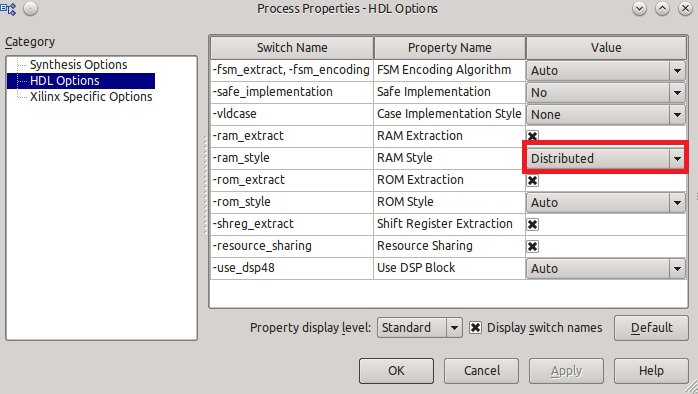
\includegraphics[scale=0.6]{figures/dut-ram-style}
		\caption{\label{fig:dut-ram-style}DUT RAM Style}
		\end{center}
		\vspace{-3ex}
		\end{figure}
     \end{enumerate}
  \item Set the \texttt{dutTopLevel} as the top-level module in this project.
		\begin{figure}[H]
		\begin{center}
		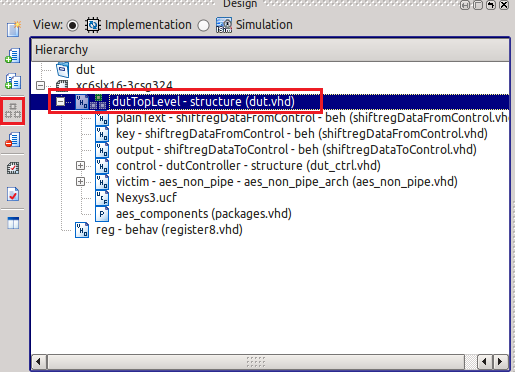
\includegraphics[scale=0.6]{figures/dut-set-top-level}
		\caption{\label{fig:dut-set-top-level}Set DUT Top-level}
		\end{center}
		\vspace{-3ex}
		\end{figure}
  \item Generate the programming bit file for the DUT by clicking "Generate Programming File" in the Processes window.
  \item Program the DUT using Xilinx Impact. In the Processes window, click Configure Target Device (See Fig~\ref{fig:dut-run-impact}).
		\begin{figure}[H]
		\begin{center}
		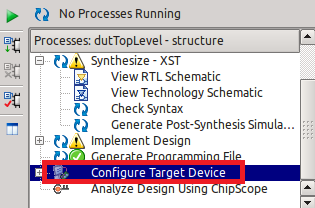
\includegraphics[scale=0.6]{figures/dut-run-impact}
		\caption{\label{fig:dut-run-impact}}
		\end{center}
		\vspace{-3ex}
		\end{figure}
  \item In the Impact window, click "Boundary Scan" then form the File menu, click "Initialize Chain" and assign the bit file to the FPGA. Now you may right-click the FPGA and click "Program".
		\begin{figure}[H]
		\begin{center}
		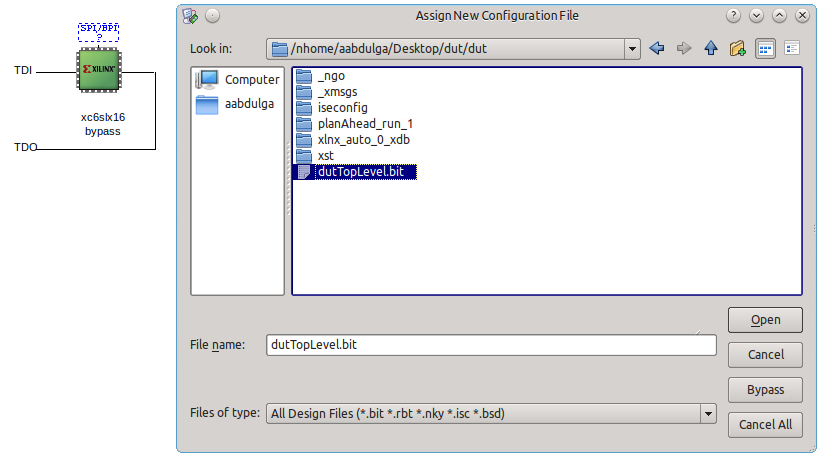
\includegraphics[scale=0.6]{figures/dut-program}
		\caption{\label{fig:dut-program}Progrmamming DUT}
		\end{center}
		\vspace{-3ex}
		\end{figure}
  \end{enumerate}
\item \textbf{Connect hardware}
  \begin{enumerate}
  \item Connect control board to power and ground.
  \item Connect control board tirgger output to channel 2 on the oscilloscope.
  \item Connect the control board to the DUT using the bridge connector.
  \item Connect the control board to the PC running the FOBOS software using USB.
  \item Connect clock generator to the bridge connector. Set the clock generator clock to 600 KHz.
  \item Connect the current probe to channel 1 on the oscilloscope.
  \item Connect the current probe to the DUT's ground.
  \item Connect DUT to power making sure that the current probe is measuring the current.
  \item Connect DUT to power supply ground.
  \end{enumerate}
\item \textbf{Run FOBOS Capture}
  \begin{enumerate}
  \item In console type:
    \texttt{cd \$fobos/bin}
  \item Edit the texttt{\$fobos/config/acquisitionConfig.txt} fil to look like the following (Make sure to set OSCILLOSCOPE\_IP and OSCILLOSCOPE\_PORT to correct values) :
    

    \begin{figure}[H]
    \begin{Verbatim}[frame=single]
# =============================================
# Global Settings
# =============================================
MEASUREMENT_FORMAT = dat # Default => dat
LOGGING = INFO # INFO|DEBUG
# =============================================
# Control Board Settings
# =============================================
CONTROL_BOARD = Nexys2
VICTIM_RESET = 11
TIME_OUT = 50000
TRIGGER_WAIT_CYCLES = 1 #@VICTIM CLOCK must be >0
TRIGGER_LENGTH_CYCLES = 1 #@VICTIM CLOCK
# =============================================
# Test Data Generation Settings
# =============================================
PLAINTEXT_GENERATION = RANDOM # USER | RANDOM
DATA_FILE     = plaintexts.txt
KEY_GENERATION = RANDOM # USER | RANDOM 
KEY_FILE      = keys.txt
INPUT_FORMAT  = hex # Default => hex
OUTPUT_FORMAT = hex # Default => hex
NUMBER_OF_ENCRYPTIONS_PER_TRACE = 1
BLOCK_SIZE = 16 # In Bytes
KEY_SIZE = 16 # In Bytes
# =============================================
# FOBOS Capture Settings
# =============================================
DUMMY_RUN = NO  #YES/NO
NUMBER_OF_TRACES = 20
####################################################
######## Signal Alignment Module Parameters ########
####################################################
CAPTURE_MODE = SINGLE # MULTI|SINGLE
TRIGGER_THRESHOLD = 1.0
# =============================================
# FOBOS Oscilloscope Settings
# ============================================
# INTIALIZATION OPTIONS
OSCILLOSCOPE = AGILENT #AGILENT|OPENADC
OSCILLOSCOPE_IP = 192.168.0.10
OSCILLOSCOPE_PORT = 5025
AUTOSCALE = NO   # YES|NO    
IMPEDANCE = FIFTY #FIFTY|ONEMEG
# VOLTAGE AND TIME RANGE OPTIONS        
CHANNEL1_RANGE = 0.12V
CHANNEL2_RANGE = 6V
CHANNEL3_RANGE = OFF # ON|OFF|voltage range
CHANNEL4_RANGE = OFF # ON|OFF|voltage range
TIME_RANGE = 0.000028
TIMEBASE_REF = LEFT    
# TRIGGER OPTIONS
TRIGGER_SOURCE =  CHANNEL2
TRIGGER_MODE =  EDGE   
TRIGGER_SWEEP = NORM
TRIGGER_LEVEL = 1
TRIGGER_SLOPE = POSITIVE
# ACQUIRE OPTIONS
ACQUIRE_TYPE = NORM # NORM|PEAK|HRES|AVER
ACQUIRE_MODE = RTIM   # RTIM | ETIM| SEG
      \end{Verbatim}
      \caption{\label{fig:fobos:acqconf}Snippet of acquisitionConfig.txt}
      \end{figure}
      
      \item Run the acquisition script as follows: \texttt{python dataAcqusition.py}
      
  \end{enumerate}
 \item \textbf{Load your hypothetical power data.}
  \begin{enumerate}
   \item Copy the aes\_hw.py script from \$fobos/examples/AES-128/powermodel/ to \$fobos/FOBOSWorkspace/testing/\$attempt/output.
   \item Generte your hypothetical data. Run \texttt{python3 aes\_hw.py}
   \item Copy the hypothetical data files to the \$fobos/data/ directory.
  \end{enumerate}

\item \textbf{Run FOBOS Analysis.}
  \begin{enumerate}
   \item Edit the configuration files in the \$fobos/config directory as follows:
   
   
   \textbf{compressionParams.txt}
   \begin{figure}[H]
	\begin{Verbatim}[frame=single]
####################################################
######## Compression Module Parameters #############
####################################################
COMPRESSION_LENGTH = 10
COMPRESSION_TYPE = MEAN # MAX|MIN|MEAN
	\end{Verbatim}
	\caption{\label{fig:fobos:paramsa}Snippet Compression Parameters}
	\end{figure}
	
  
   \textbf{dataAnalysisParams.txt}
   \begin{figure}[H]
	\begin{Verbatim}[frame=single]
WORK_DIR = FOBOSAnalysis
MEASUREMENT_WORK_DIR = FOBOSWorkspace
TAG = counter
	\end{Verbatim}
	\caption{\label{fig:fobos:paramanalysis}Snippet Data Analysis Parameters}
	\end{figure}
	
   
   \textbf{dataAnalysisParams.txt}
   \begin{figure}[H]
	\begin{Verbatim}[frame=single]
####################################################
######## Post Processing Flow ######################
####################################################
SAMPLE_SPACE_DISPOSITION = 2 # 1-3|NO
COMPRESS_DATA = 3 #1-3|NO
TRACE_EXPUNGE = 1 #1-3|NO 
TRACE_EXPUNGE_PARAMS = VAR-0.0000110:0.0000139 #STD|VAR-BELOW:ABOVE|NO
	\end{Verbatim}
	\caption{\label{fig:fobos:parampsotproc}Snippet Post Processing Parameters}
	\end{figure}
	
   \textbf{sampleSpaceDispParams.txt}
   \begin{figure}[H]
	\begin{Verbatim}[frame=single]
####################################################
#### Sample Space Disposition Module Parameters ####
####################################################
SAMPLE_WINDOW_SIZE = 2000
SAMPLE_WINDOW_START = 100 
	\end{Verbatim}
	\caption{\label{fig:fobos:paramdisp}Snippet Sample Space Disposition Parameters}
	\end{figure}
	
    
   \textbf{signalAlignmentParams.txt}
   \begin{figure}[H]
	\begin{Verbatim}[frame=single]
####################################################
######## Signal Alignment Module Parameters ########
####################################################
CAPTURE_MODE = SINGLE # MULTI|SINGLE
TRIGGER_THRESHOLD = 1.0
	\end{Verbatim}
	\caption{\label{fig:fobos:paramalingn}Snippet Signal Alignment Parameters}
	\end{figure}
   
   \textbf{traceExpungeParams.txt}
   \begin{figure}[H]
	\begin{Verbatim}[frame=single]
####################################################
######## Trace Expunge Module Parameters ###########
#################################################### 
TRACE_EXPUNGE_PARAMS = VAR:0.0004:0.00045 #STD|VAR:BELOW:ABOVE|NO
	\end{Verbatim}
	\caption{\label{fig:fobos:paramexpunge}Snippet Trace Expunge Parameters}
	\end{figure}
    \item Run the Data Analysis script: \texttt{python dataAnalysis.py}
    \item Check the analysis output files in \$fobos/FOBOSWorkspace/testing/\$attempt/analysis.
  \end{enumerate}


\end{enumerate}


\end{document}
 
